%\documentclass[aps,prl,twocolumn,showpacs,superscriptaddress,groupedaddress]{revtex4}  % for review and submission
%\documentclass[aps,preprint,showpacs,superscriptaddress,groupedaddress]{revtex4}  % for double-spaced preprint
%\documentclass[aps,prl,floatfix,twocolumn,10pt]{revtex4-1}  % for review and submission
%\documentclass[aps,prl,preprint]{revtex4-1}  % for double-spaced preprint
\documentclass[aip,apl,amsmath,amssymb,floatfix,reprint,a4paper]{revtex4-1}

%% Packages
\usepackage{graphicx}  %figures
\usepackage{subfigure} %subfigures
\usepackage{amssymb}   %math
\usepackage{upgreek}   %non-italic greek letters
\usepackage[utf8]{inputenc} %Umlaute

%% hyphenation settings
\hyphenation{ALPGEN}
\hyphenation{EVTGEN}
\hyphenation{PYTHIA}

%% New commands
\newcommand{\unit}[1]{\ensuremath{\, \mathrm{#1}}}
\newcommand{\msub}[1]{\ensuremath{\textnormal{\begin{tiny}#1\end{tiny}}}}

%% ----------------------------------------------------------------------------------------------------------------
\begin{document}

\title{Compact X-ray grating interferometry at 100~keV}

\author{T.~Thüring}
  \affiliation{Paul Scherrer Institut, Villigen PSI, Switzerland}
  \affiliation{Institute for Biomedical Engineering, Swiss Federal Institute of Technology, Zurich, Switzerland}
\author{M.~Abis}
  \affiliation{Paul Scherrer Institut, Villigen PSI, Switzerland}
  \affiliation{Institute for Biomedical Engineering, Swiss Federal Institute of Technology, Zurich, Switzerland}
\author{Z.~Wang}
  \affiliation{Paul Scherrer Institut, Villigen PSI, Switzerland}
\author{C.~David}
  \affiliation{Paul Scherrer Institut, Villigen PSI, Switzerland}
\author{M.~Stampanoni}
  \affiliation{Paul Scherrer Institut, Villigen PSI, Switzerland}
  \affiliation{Institute for Biomedical Engineering, Swiss Federal Institute of Technology, Zurich, Switzerland}

\date{\today}


%% ----------------------------------------------------------------------------------------------------------------
\begin{abstract}
Today's X-ray phase contrast imaging techniques are not only limited by spatial and temporal coherence properties of the beam, but also by the applicable energy range. Imaging at higher energies is of particularly high interest as it would vastly expand the range of applications, for instance, by the possibility to examine materials of higher density or thickness. Grating interferometry, albeit proven to be one of the most promising methods for the industrial applicability of phase and dark field contrast imaging, is limited to energies to about $50 \unit{keV}$ due to the lack of a grating manufacturing grating technology for sufficiently high aspect ratios. We herein propose an alternative approach, which enables the access to the entire diagnostic energy range of X-rays for phase and dark field contrast imaging on compact systems with low brilliance X-ray tubes. Based on Talbot-Lau interferometry, the novel approach involves the edge-on illumination of specially designed gratings, solving two fundamental problems at once. First, the effective aspect ratio is not determined or limited by the structure height limitation of the manufacturing technology and thus, arbitrary aspect ratios are feasible. Secondly, the intrinsic reduction of the field of view for higher aspect ratios is solved by a circular alignment of the edge-on illuminated grating structures. Based on this, a compact Talbot-Lau interferometer has been set up with a design energy at $100 \unit{keV}$, providing 2D and 3D phase and dark field contrast images of dense materials. The approach is not only applicable to X-rays, but is also compatible to other grating based imaging modalities such as neutrons.
\end{abstract}


\maketitle

%%%%%%%%%%%%%%%%%%%%%%%%%%%%%%%%%%%%%%%%%%%%%%%%%%%%%%%%%%%%%%%%%%%%%%%%
% Body of manuscript
%%%%%%%%%%%%%%%%%%%%%%%%%%%%%%%%%%%%%%%%%%%%%%%%%%%%%%%%%%%%%%%%%%%%%%%%

X-ray radiography and computed tomography (CT) are nowadays standard imaging techniques for the non-destructive testing of materials or for medical diagnosis in daily routine. The physical contrast mechanism relies on the attenuation of X-rays in an object through the photo-electric effect or Compton scattering, whereas two materials can be distinguished due to their different attenuation properties. Apart from the attenuation, the wave and particle nature of X-rays reveal two further physical interaction mechanisms that occur if an object is exposed to X-rays.

Regarding the wave properties, an interface of two different materials in an object causes a change in the wave's phase velocity and thus in a net change of the output phase (a phase shift) downstream of the object. Since no detection device is able to measure a phase shift directly, advanced techniques are necessary to obtain access to this signal.

Regarding the particle properties of X-rays, photons are randomly scattered on small structures in the material. Depending on the imaging system (geometry and energy), wide angle and small angle scattering represent typical sources of noise in absorption imaging. For the type of scattering which occurs exclusively in forward direction and under ultra small angles (order of nano radiants), the particles usually remain within the area of a detector pixel and thus this effect cannot directly be detected with standard techniques.

The main interest in the detectability of those additional interaction mechanisms is the fact that attenuation, phase shift and scattering are physically complementary interaction mechanisms, in the sense that their occurrence is mutually independent. In the context of information content of images, this gives rise to hypothesize that the complementary interaction mechanisms may eventually yield complementary image information, manifested by the image contrast.

Since currently available phase contrast techniques rely on secondary physical effects, such as interference, and thus typically on optical hardware (e.g. crystals, gratings), they vary a lot in terms of sensitivity, practical applicability or achievable resolution. The vast majority of the methods, including crystal analyzer based \cite{Davis1995,Chapman1997} or interferometric \cite{Bonse1965,Momose1996} methods rely on X-ray beams of high spatial and temporal coherence, available only at synchrotrons. Techniques with a high degree of spectral acceptance are the in-line phase contrast method \cite{Snigirev1995,Wilkins1996,Cloetens1996} and Talbot interferometry \cite{Cloetens1997,David2002,Momose2003a}. Regarding the acceptance of X-ray beams with low temporal and spatial coherence, Talbot-Lau interferometry \cite{Pfeiffer2006} and coded apertures \cite{Munro2012} are currently the only feasible techniques.

While current phase contrast methods are today broadly available on synchrotrons and constantly improving on conventional X-ray tubes, the applicable energy range is still limited to the lower diagnostic energy range ($5 - 50 \unit{keV}$). None of the reported methods is compatible to industrial or medical applications where higher X-ray energies ($>50 \unit{keV}$) are required. For instance, the portability of Talbot-Lau interferometry towards medical imaging such as chest or abdominal radiography or CT, which require energies up to $150 \unit{keV}$, has still been impossible due to the technical limitations in grating fabrication for X-ray energies higher than approx. $50 \unit{keV}$. Grating manufacturing methods are well established for energies up to about $E=40 \unit{keV}$, which partly explains the reported successes of the technique in mammography \cite{Stampanoni2011} or hand imaging \cite{Thuering2013a}. The limiting factor for currently available grating fabrication techniques is the aspect ratio $\textnormal{AR} = 2h/p$, where $p$ is the grating period and $h$ the structure height. For a given setup distance and for $p \propto 1/\sqrt{E}$ and $h \propto E^3$, it can be shown that $\textnormal{AR} \propto E^{7/2}$. While for $25 \unit{keV}$, an aspect ratio for the absorption grating of around $\textnormal{AR}=30$ is necessary for a reasonable setup length, it would have to be at least 128 for $100 \unit{keV}$. This is only approximate and ignores absorption edges of the materials (e.g., at around $80 \unit{keV}$ for gold in an absorption grating). Furthermore, when using a polychromatic spectrum, photons above the design energy should also be efficiently attenuated by the gratings to guarantee their contribution to the signal, which requires even higher aspect ratios. The current technical limitation is at $\textnormal{AR} \approx 50$, whereas such high values are often even beyond the limits and come at the expense of a poor grating quality and performance.

We herein propose an alternative design method of X-ray Talbot-Lau grating interferometers, which allows phase contrast and dark field imaging with low brilliance X-ray tubes at arbitrarily high energies. The approach is based on the edge-on illumination of gratings. Edge-on illumination, as opposed to the standard face-on illumination, exploits the arbitrary length of the grating lines to form high aspect ratios of the structures along the beam direction. Since the effective structure height of the grating is then determined by the grating dimension, the aspect ratio can be arbitrarily high. FIG.~\ref{Fig:schematic} illustrates the edge-on illumination approach.
\begin{figure} [ht]
  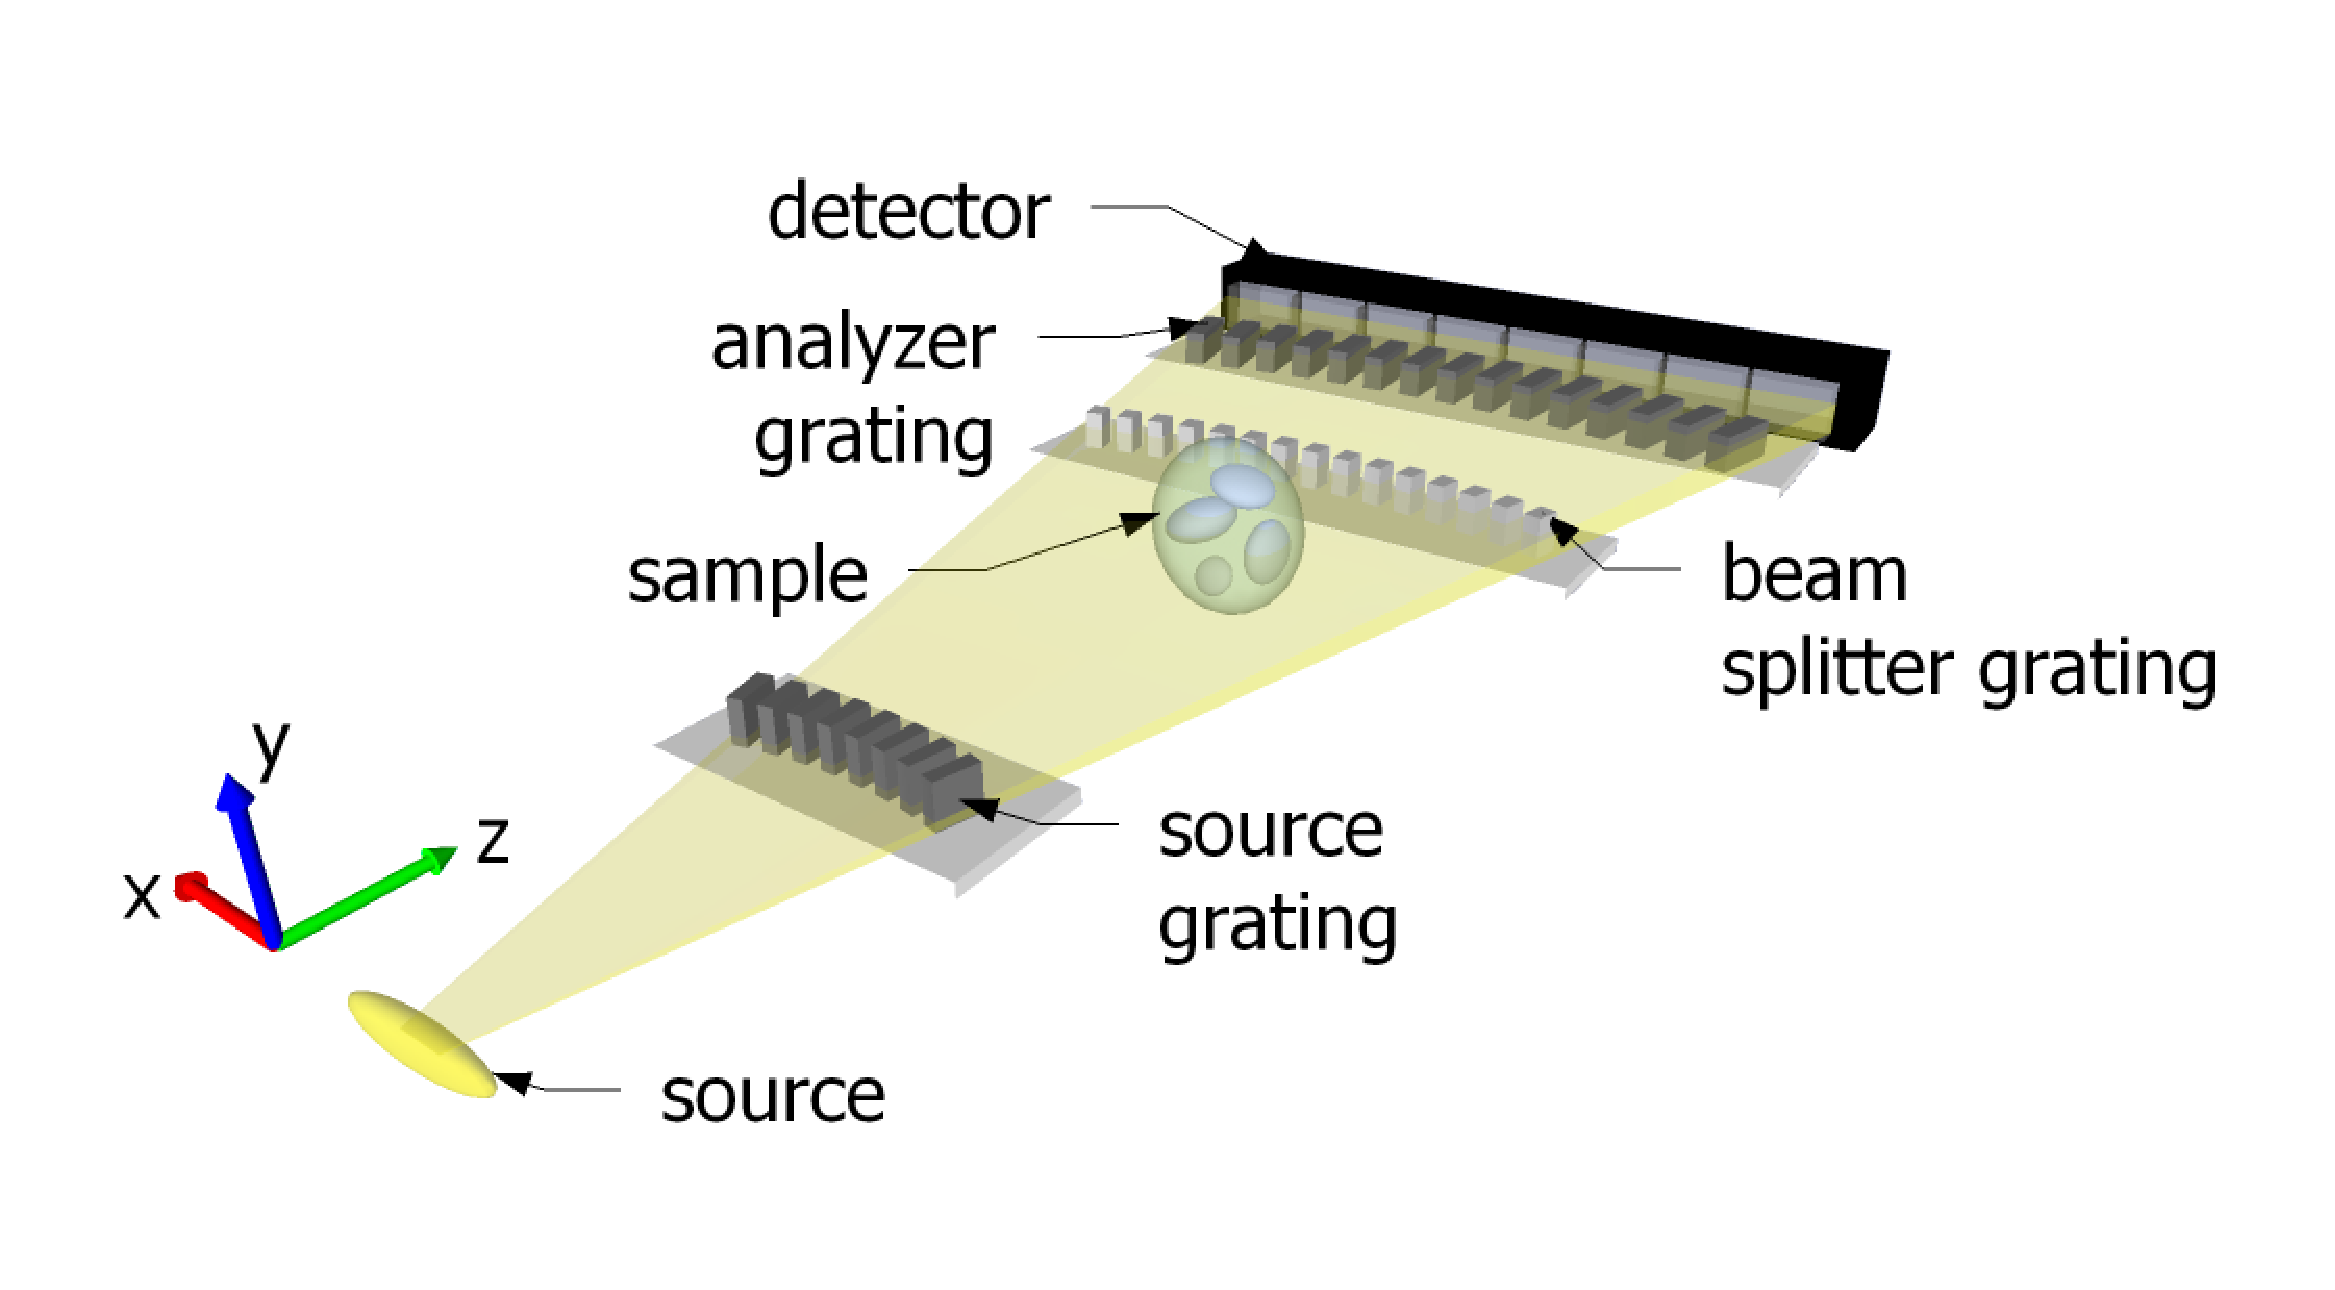
\includegraphics[width = \linewidth]{figures/figure1.eps}
  \caption{Schematic of a grating interferometer for high X-ray energies in edge-on illumination mode. The aspect ratio is defined by the ratio of the travelling distance along the grating lines and the period and can be arbitrarily long. In order to avoid a reduction of the field of view, the gratings structures aligned on an arc.}
  \label{Fig:schematic}
\end{figure}

Increasing the effective aspect ratio of the gratings typically leads to a reduction of the field of view due to the change of the transmission function at high incident angles, which has also been demonstrated by using a glancing angle of the gratings between zero and $90$ degrees \cite{Stutman2012a}. In order to overcome this problem in edge-on illuminated grating interferometry, the grating lines are aligned on an arc with a radius equal to the distance from the source to the grating (FIG.~\ref{Fig:schematic}).

The combination of edge-on illumination and the circularly curved structure alignment allows the design of a grating interferometer at any design energy in the diagnostic energy range of X-rays. The arbitrary aspect ratio only comes at the expense of a limited field of view in the vertical dimension of the image plane, which is, depending on the detector, typically a few pixels. However, radiographic 2D images can still be acquired in sample scanning mode without increasing dose. Similarly, for tomographic images, the approach allows single slice CT or full 3D imaging in scanning mode.

Gratings were manufactured by Micro Works GmbH, Germany, using a LIGA process \cite{Kenntner2010}. The grating design and fabrication is non-standard and involves a complex mask design, as shown in FIG.~\ref{Fig:grating_mask}. Each grating resides on a $5 \times 60 \unit{mm^2}$ silicon chip and has its specific structure length and curvature. Several grating chips can be fabricated on a single 4 inch silicon wafer. For the present experiments, a symmetric interferometer with a grating period of $p = 2.8 \unit{\upmu m}$ for all gratings has been used. The design energy is $100 \unit{keV}$ and the beam splitter grating periodically shifts the phase by zero and $\pi$ at this energy. Using gold as the phase shifting material, this requires a structure length of $b = 19.8 \unit{\upmu m}$. The analyzer grating is an absorption mask for sensing the changes of the interference pattern generated by the beam splitter. With a structure length of $b = 800 \unit{\upmu m}$, this grating has an aspect ratio of approx. 570 and thus sufficiently attenuates X-rays up to energies of around $160 \unit{keV}$. Beam splitter- and analyzer grating are separated at the first fractional Talbot order and the distance from the source grating to the analyzer grating is $32 \unit{cm}$. The source grating is positioned $23 \unit{cm}$ away from the source and has the structure length is also  $800 \unit{\upmu m}$.
\begin{figure} [ht]
  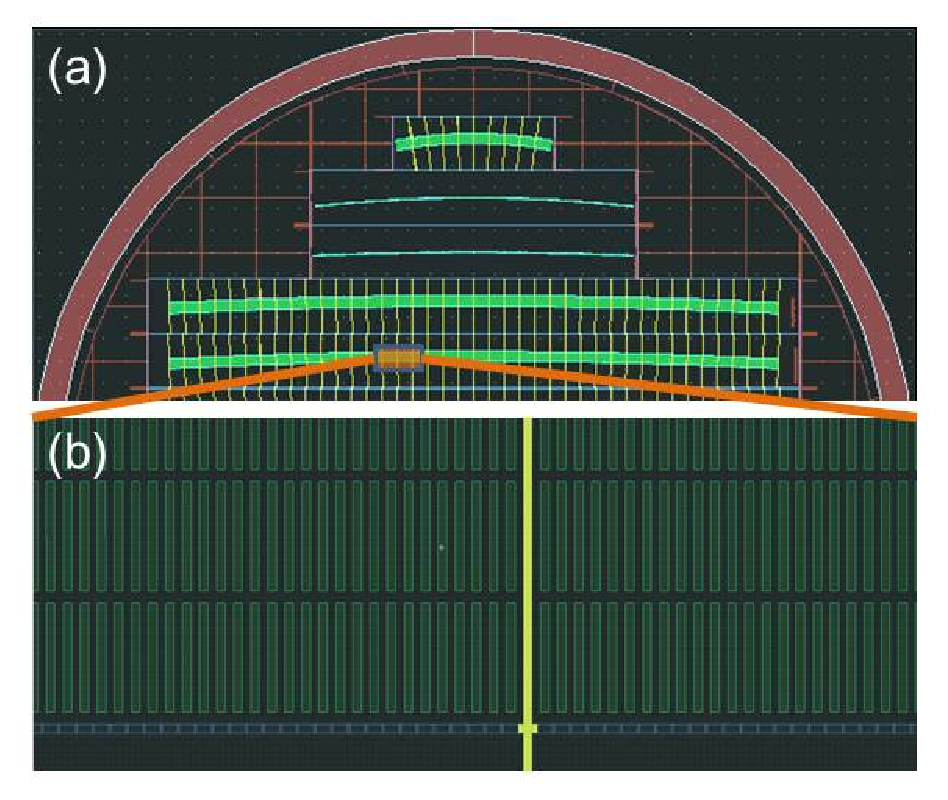
\includegraphics[width = \linewidth]{figures/grating_mask.eps}
  \caption{Grating design mask for the edge-on illumination approach. (a) Top part of the 4 inch wafer, showing five grating chips; one source grating, two beam splitter gratings and two analyzer gratings (from top to bottom). The gratings have different curvatures which are specific to the grating interferometer geometry. (b) Zoom into the grating structures, contain interrupting bridges used for stabilizing the grating structures in the LIGA process.}
  \label{Fig:grating_mask}
\end{figure}

The X-ray source is a COMET MXR-160HP/11 X-ray tube with a maximum output voltage of $160 \unit{kV}$. Since the absorption gratings perform efficiently up to $160 \unit{keV}$ and the spectral acceptance at the first fractional Talbot order is high ($50 \unit{keV}$ to $>160 \unit{keV}$), the tube voltage was set to the maximum of $160 \unit{kV}$ and operated at a current of $10 \unit{mA}$. The focal spot size is approx. $1 \unit{mm}$. The detector is a CCD camera from Finger Lakes Instruments. A cesium iodide (CsI) scintillator of $600 \unit{\upmu m}$ thickness converts the X-rays to visible light and is coupled with an optical lens projecting the image onto the CCD. The effective pixel size is $80 \unit{\upmu m}$. With a grating structure height of approx. $100 \unit{\upmu m}$, the field of view in the vertical direction is limited to one pixel row. In addition to the standard components (source, camera, interferometer), two optical slit, one in front of the source grating, the other in front of the camera, have been installed for the collimation of the beam in vertical direction. X-rays which are not travelling through all of the gratings do not contribute to the signal and are attenuated by the slits. The slit widths are $25 \unit{\upmu m}$ and $100 \unit{\upmu m}$, respectively.

FIG. 3 shows a radiographic image of a metal screw in all three contrast modes, acquired with the $100 \unit{keV}$ setup. Grating interferometry at such a high diagnostic energy allows to examine more dense materials such as metals in phase contrast mode. At lower energies, the phase shifts of such materials would be too large and wrap over multiple periods of the analyzer grating.


Edge-on illuminated grating interferometry breaks the current limitation to the low diagnostic energy range for X-ray phase contrast imaging with conventional X-ray sources. Compact geometries for design energies well above 100 keV can be realized for the examination of dense materials which would be intransparent at lower energies of currently used phase contrast techniques. The approach is not limited to X-ray imaging, it can also be applied to other grating based imaging modalities (e.g., with neutrons \cite{Grunzweig2008}) where high aspect ratios are necessary.

We thank Gordan Mikuljan from Paul Scherrer Institute, Switzerland, for his work on the mechanical design, Joachim Schulz and Marco Walter from Micro Works GmbH, Germany, for the competent support on grating design issues, Christian Kottler and Vincent Revol from Centre Suisse d'Electronique et de Microtechnique (CSEM), Switzerland for the fruitful discussions on grating interferometer design.



\bibliography{library.bib}
\bibliographystyle{apsrev4-1}

\end{document}